\begin{adjustwidth*}{}{-2.25in}
\textbf{{\large Exercises}}
\setlength{\columnsep}{25pt}
\begin{multicols*}{2}
\noindent Terms and Concepts \small
\begin{enumerate}[1)]
\item What is the name of the rule which states that $\ds \frac{d}{dx}\big(x^n\big) = nx^{n-1}$, where $n>0$ is an integer?
\item Give an example of a function $f(x)$ where $f'(x) = f(x)$.
\item Give an example of a function $f(x)$ where $f'(x) = 0$.
\item The derivative rules introduced in this section explain how to compute the derivative of which of the following functions?

\setlength{\columnsep}{15pt}
\bmtwo
\ba
\item $\ds g(x) = 3x^2-x+17$ 
\item $\ds h(x) = 5\ln(x)$ 
\item $\ds j(x) = \sin(x) \cos(x)$ 
\item $\ds k(x) = e^{x^2}$
\item $\ds m(x) = \sqrt{x}$
\item $\ds f(x) = \frac{3}{x^2}$ 
\ea
\emtwo
\setlength{\columnsep}{25pt}
\end{enumerate} 

\noindent {\normalsize Problems} \small

\noindent {\bf In exercises 5--13, compute the derivative of the given function.}

\begin{enumerate}[1),resume]
\item $\ds f(x) = 7x^2-5x+7$
\item $\ds g(x) = 14x^3+7x^2+11x-29$
\item $\ds m(t) = 9t^5-\frac{1}{8}t^3+3t-8$
\item $\ds f(\theta) = 9\sin(\theta) + 10\cos(\theta)$
\item $\ds f(r) = 6e^r$
\item $\ds g(t) = 10t^4-\cos(t) +7\sin(t)$
\item $\ds p(s) = \frac{1}{4}s^4+\frac{1}{3}s^3+\frac{1}{2}s^2+s+1$
\item $\ds h(t) = e^t - \sin(t) - \cos(t)$
\item $\ds g(t) = (1+3t)^2$
\end{enumerate}

\noindent {\bf In exercises 14--19, compute the first four derivatives of the given function.}

\begin{enumerate}[1),resume]
\item $\ds f(x) = x^6$
\item $\ds g(x) = 2\cos(x)$
\item $\ds h(t) = t^2 - e^t$
\item $\ds p(\theta) = \theta^4-\theta^3$
\item $\ds f(\theta) = \sin(\theta)-\cos(\theta)$
\item $f(x)=1,100$
\end{enumerate}

\noindent {\bf In exercises 20--24, find the equation of the tangent line of the function at the given point.}

\begin{enumerate}[1),resume]
\item $\ds f(x)=x^3-x$ at $x=1$
\item $\ds f(t)=e^t+3$ at $t=0$
\item $\ds f(x)=4\sin(x)$ at $x=\pi/2$
\item $\ds f(x)=-2\cos(x)$ at $x=\pi/4$
\item $\ds f(x)=2x+3$ at $x=5$

\item Let $f$ and $g$ be differentiable functions for which the following information is known:  $f(2) = 5$, $g(2) = -3$, $f'(2) = -1/2$, $g'(2) = 2$.
\ba
	\item Let $h$ be the new function defined by the rule $h(x) = 3f(x) - 4g(x)$.  Determine $h(2)$ and $h'(2)$.
	\item Find an equation for the tangent line to $y = h(x)$ at the point $(2,h(2))$.
	\item Let $p$ be the function defined by the rule $p(x) = -2f(x) + \frac{1}{2}g(x)$.  Is $p$ increasing, decreasing, or neither at $a = 2$?  Why?
	\item Estimate the value of $p(2.03)$ by using the local linearization of $p$ at the point $(2,p(2))$.
\ea

\item Consider the functions $r(t) = t^t$ and $s(t) = \arccos(t)$, for which you are given the facts that $r'(t) = t^t(\ln(t) + 1)$ and $s'(t) = -\frac{1}{\sqrt{1-t^2}}$.  Do not be concerned with where these derivative formulas come from.  We restrict our interest in both functions to the domain $0 < t < 1$.
\ba
	\item Let $w(t) = 3t^t - 2\arccos(t)$.  Determine $w'(t)$.
	\item Find an equation for the tangent line to $y = w(t)$ at the point $(\frac{1}{2}, w(\frac{1}{2}))$.
	\item Let $v(t) = t^t + \arccos(t)$.  Is $v$ increasing or decreasing at the instant $t = \frac{1}{2}$?  Why?
\ea

\item Let functions $p$ and $q$ be the piecewise linear functions given by their respective graphs given below.  Use the graphs to answer the following questions.
\begin{center}
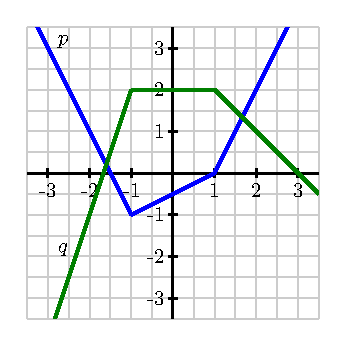
\includegraphics[scale=.7]{figures/2_1_Ez3.eps}
\end{center}
\ba
	\item At what values of $x$ is $p$ not differentiable?  At what values of $x$ is $q$ not differentiable? Why?
	\item Let $r(x) = p(x) + 2q(x)$.  At what values of $x$ is $r$ not differentiable? Why?
	\item Determine $r'(-2)$ and $r'(0)$.
	\item Find an equation for the tangent line to $y = r(x)$ at the point $(2,r(2))$.
\ea

\item Use the definition of the derivative to prove the Constant Rule for differentiation. \label{E:2.4-45}

\item Use the definition of the derivative to prove the Constant Multiple Rule for differentiation. \label{E:2.4-46}

\item Use the definition of the derivative to prove the Sum Rule for differentiation. \label{E:2.4-47}
\end{enumerate}

%------------------------------------------
% END OF EXERCISES ON FIRST PAGE
%------------------------------------------
\end{multicols*}
\end{adjustwidth*}

\afterexercises